% By default, the contents of the back side of the final sheet is
% printed upside down. The option notumble suppresses that. Doing so
% may be necessary to suit the behavior of certain printing engines.
% Specifying [notumble] may also be useful during the writing of a
% document, to enable proof-reading on the screen.
\documentclass[notumble]{leaflet}
%\documentclass{leaflet}


\usepackage[english]{babel}
\usepackage[utf8]{inputenc}
\usepackage{lmodern}
\usepackage[T1]{fontenc}

\usepackage[default,scale=.82]{opensans}
% \renewcommand{\seriesdefault}{cl}
\renewcommand{\bfdefault}{sb}
% \renewcommand{\ttdefault}{fos}
\renewcommand\ttfamily{%
  \fontfamily{\ttdefault}%
  % \fontseries{lc}%
  \fontshape{\shapedefault}%
  \selectfont}

\usepackage{enumitem}
\setlist{
    topsep=0pt,
    partopsep=0pt,
    parsep=1ex,
    nolistsep,
    itemsep=.5ex
}
\setlength{\parskip}{.5\smallskipamount}

\usepackage[table,svgnames]{xcolor}
\usepackage{graphicx}
\usepackage{tabularx,booktabs}
\usepackage{alltt,textcomp}
\usepackage{url}
\urlstyle{sf}
\usepackage{ifthen}
\usepackage{xspace}

\newcommand{\eg}{\emph{e.g.,}\xspace}
\newcommand{\ie}{\emph{i.e.,}\xspace}
\newcommand{\etal}{\emph{et al.,}\xspace}
\newcommand{\ct}[1]{{\textsf{#1}}\xspace}

\usepackage{microtype}

\makeatletter
\newsavebox{\code@box}
\definecolor{light-gray}{rgb}{0.9,0.9,0.9}
\newenvironment{displaycode}{%
    \par
    \begin{lrbox}{\code@box}%
        \begin{minipage}{\linewidth}
            \begin{alltt}\small}{
            \end{alltt}
        \end{minipage}
    \end{lrbox}
    \colorbox{light-gray}{\usebox{\code@box}}%
    \par}
%\let\code\texttt
% Use of english prevents babel from adding spaces before $:
\newcommand{\code}[1]{\foreignlanguage{english}{\texttt{#1}}}
\makeatother


\graphicspath{{./figures/}}

\title{%
  % \fontseries{cl}\selectfont\huge
  % Cheat sheet\\
  \vspace*{0.5\textwidth}%
  \normalfont
  
\includegraphics[width=\linewidth]{logo.pdf}
  \\[1.8\baselineskip]%
  \fontseries{cl}\selectfont\Huge
  a clean, innovative, open-source Smalltalk-inspired environment\\
  \vfill
  \url{http://www.pharo.org}}

\date{}

\CutLine*{1} \CutLine*{2} \CutLine*{3} \CutLine*{4} \CutLine*{5}
\CutLine*{6}


\begin{document}
\maketitle
\thispagestyle{empty}

\pagebreak{}

\section{Pharo: the Elevator Pitch}

Pharo is both an \emph{object-oriented}, \emph{dynamically-typed}
general-purpose language and its own programming environment. The
language has a simple and expressive syntax which can be learned
in a few minutes. Concepts in Pharo are \emph{very consistent}:
\begin{itemize}
  \item Everything is an object: buttons, colors, arrays, numbers, classes, methods\ldots \emph{Everything!}
  \item A small number of rules, no exceptions!
\end{itemize}

Pharo runs in a \emph{virtual machine}. Development takes place in an
\emph{image} in which all objects live and can be modified. The state
of an image can be saved and reloaded later to get all your objects
and tools back. Image-based development feels really different from
file-based development.

% Not enough space for that :-( Extracting the source code from the
% image is done through a dedicated version control system; publishing
% code can be done on open servers such as
% \url{http://smalltalkhub.com}.

\subsection{Minimal Syntax}

\noindent
\begin{tabularx}{\linewidth}{@{}rX@{}}
        \toprule
        \multicolumn{2}{c}{Six reserved words only}\\
        \midrule
        \code{nil} & the undefined object\\
        \code{true}, \code{false} & boolean objects\\
        \code{self} & the receiver of the current message\\
        \code{super} & the receiver, in the superclass context\\
        \code{thisContext} & the current invocation on the call stack\\
        \addlinespace

        \toprule
        \multicolumn{2}{c}{Reserved punctuation characters}\\
        \midrule
        \code{"}{comment}\code{"} & \\
        \code{'}{string}\code{'} & \\
        \code{\#symbol} & unique string \\
        \code{\$a} & the character \code{a} \\
        \code{12 2r1100 16rC} & twelve (decimal, binary, hexadecimal)\\
        \code{3.14 1.2e3} & floating-point numbers\\
        \code{.} & expression separator (period)\\
        \code{;} & message cascade (semicolon)\\
        \code{:=} & {assignment} \\
        \code{\textasciicircum} & return a result from a method (caret)\\
        \code{[\,:p\,|\,}\emph{expr}\code{\,]} & code block with a parameter \\
        \code{|\,foo bar\,|} & declaration of two temporary variables \\
        \code{\#(abc 123)} & literal array with the symbol \code{\#abc} and the number \code{123} \\
        \code{\{foo\,.\ 3\,+\,2\}} & dynamic array built from 2 expressions\\
        \bottomrule
\end{tabularx}

\subsection{Message Sending}

A method is called by sending a message to an object, the message
\emph{receiver}; the message returns an object. Messages are modeled
from natural languages, with a subject, a verb, and complements. There
are three types of messages: unary, binary, and keyword.

\paragraph{Unary Messages.}

A unary message is one with no arguments.

\begin{displaycode}
Array new.
#(1 2 3) size.
\end{displaycode}

The first example creates and returns a new instance of the
\code{Array} class, by sending the message \code{new} to the class
\code{Array} (that is an object). The second message returns the size
of the literal array which is \code{3}.

\paragraph{Binary Messages.}

A binary message takes only one argument and is named by one or more
symbol characters.

\begin{displaycode}
3 + 4.
'Hello', ' World'.
\end{displaycode}

The \code{+} message is sent to the object \code{3} with \code{4} as
the argument. In the second case, the string \code{'Hello'} receives the message \code{,} (comma) with \code{'~World'} as the argument.

\paragraph{Keyword Messages.}

A keyword message can take one or more arguments that are inserted in
the message name.

\begin{displaycode}
'Smalltalk' allButFirst: 5.
3 to: 10 by: 2.
\end{displaycode}

The first example sends the message \code{allButFirst:} to a string,
with the argument \code{5}. This returns the string
\code{'talk'}. The second example sends \code{to:by:} to
\code{3}, with arguments \code{10} and \code{2}; this
returns a collection containing \code{3}, \code{5}, \code{7},
and \code{9}.

\paragraph{Precedence.}

Parentheses\,$>$\,unary\,$>$\,binary\,$>$\,keyword, and finally from left to right.

\begin{displaycode}
(10 between: 1 and: 2\,+\,4\,*\,3) not
\end{displaycode}

Here, the messages \code{+} and \code{*} are sent first, then \code{between:and:} is sent, and finally \code{not}.
The rule suffers no exception: operators are just binary messages with \emph{no notion of mathematical precedence}, so
\code{2\,+\,4\,*\,3} reads left-to-right and gives 18, not 14!

\subsection{Message Cascade}

Multiple messages can be sent to the same receiver with \code{;}.

\begin{displaycode}
OrderedCollection new
  add: #abc;
  add: #def;
  add: #ghi.
\end{displaycode}

The message \code{new} is sent to \code{OrderedCollection} which
results in a new collection to which 3 \code{add:} messages are sent.
The value of the whole message cascade is the value of the last
message sent (here, the symbol \code{\#ghi}). To return the receiver
of the message cascade instead (\ie the collection), make sure to send
\code{yourself} as the last message of the cascade.

\subsection{Blocks}

Blocks are objects containing code that is executed on demand,
(anonymous functions). They are the basis for control structures like
conditionals and loops.

\begin{displaycode}
2 = 2 ifTrue: [Error signal: 'Help'].
\#('Hello World' \$!) do: [:e | Transcript show: e]
\end{displaycode}
The first example sends the message \code{ifTrue:} to the boolean
\code{true} with a block as argument. Because the boolean is
\code{true}, the block is executed and an exception is signaled. The
next example sends the message \code{do:} to an array. This evaluates
the block once for each element, passing it via the \code{e}
parameter. As a result, \code{Hello~World!} is printed.

\section{Pharo: a Live Programming Environment}

Pharo comes with an integrated development environment that allows you
to browse not only your source code, but also the whole system. Pharo
is a \emph{live programming environment}: you can modify your objects
and your code while your program is executing. All Pharo tools are
implemented in Pharo:
\begin{itemize}
\item a code browser with refactoring tools;
\item a workspace and object inspectors;
\item a debugger;
\item a version control system;
\item and much, much more!
\end{itemize}

Code can be inspected and evaluated directly in the image, using
simple key combinations and menus (right click on any selected text to
see available options).

\begin{center}
  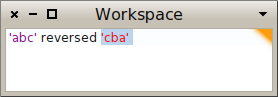
\includegraphics[width={.6}\textwidth]{workspace}
\end{center}

\clearpage
\subsection{The Pharo Code Browser}

The Pharo code browser is composed of 5 panes:

\begin{itemize}
\item The \emph{packages} pane shows all the packages of the system or
  just a subset (by \emph{scoping} the browser);
\item The \emph{classes} pane shows a hierarchy of the classes in the
  selected package; in gray, the classes that are extended in the
  selected package but that belong to another one; the \emph{class
    side} checkbox allows for getting the methods of the meta-class of
  the selected class; the \emph{comments} button toggles the display
  of the current class's comment;
\item The \emph{protocols} pane groups the methods in the selected
  class; protocols facilitate searching for a method when the
  developer does not know its name; a protocol whose name starts with a
  \emph{*} (star) groups methods that belong to a different package
  than the one of the selected class (\eg the
  \emph{*Morphic-Basic} protocol groups methods that belong
  to the \emph{Morphic-Basic} package);
\item The \emph{methods} pane lists the methods of the selected
  protocol (or of the class if no protocol is selected); a down-arrow
  icon in front of a method indicates a method overridden in at least
  one subclass; an up-arrow icon indicates that the current method
  overrides one from the superclass; icons are clickable and trigger
  dedicated actions based on their meanings;
\item The \emph{source code} pane shows the source code of the select
  method; the first 3 icons on the right allows for seeing the source
  code (\emph{S}), bytecode (\emph{B}), and decompiled code
  (\emph{D}); the following 2 icons allows for finding usages of
  instance and class variables (\emph{I} and \emph{C}).
\end{itemize}

\begin{center}
  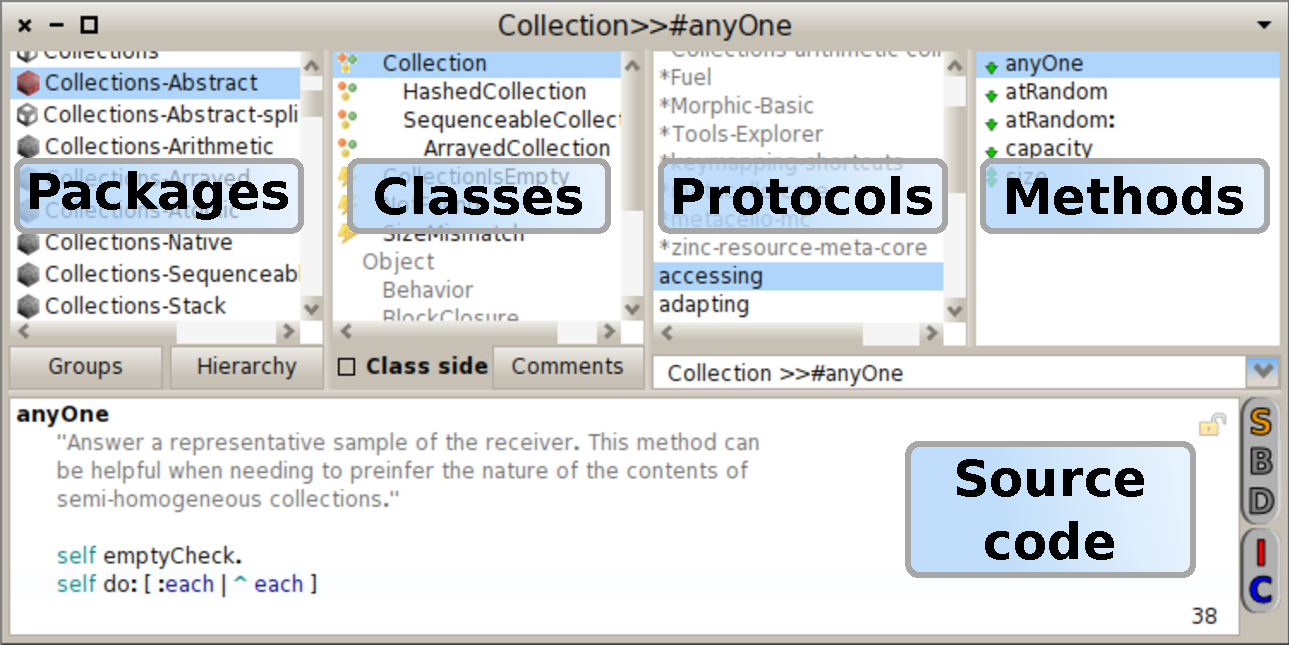
\includegraphics[width={1}\textwidth]{nautilus-anotated}
\end{center}

\pagebreak{}

\vspace*{\fill}

\section{Books}


\begin{description}
\item[Pharo By Example]
  (also available through amazon.com)\\
  \url{http://pharobyexample.org}
\item[Deep into Pharo]
  (soon to be released)\\
  \url{https://ci.inria.fr/pharo-contribution/job/DeepIntoPharo}
\item[More related books]~\\
    \url{http://stephane.ducasse.free.fr/FreeBooks}
\end{description}



\section{Links}

\begin{description}
\item[Main website] \url{http://www.pharo.org}
\item[Code hosting] \url{http://smalltalkhub.com}
\item[Questions] \url{http://stackoverflow.com/questions/tagged/pharo}
\item[Consortium] \url{http://consortium.pharo.org}
\item[Association] \url{http://association.pharo.org}
\end{description}

\vfill{}

\end{document}

%%% Local Variables:
%%% mode: latex
%%% TeX-master: t
%%% End:
